\section{Approach}
\label{sec:approach}
We present an ICL strategy in the context of the vanilla sequence-to-sequence (Seq2Seq) 
training objective with a detailed learning algorithm.
%We first present the idea of ICL in the context of the
%vanilla sequence-to-sequence(Seq2Seq) training objective. 
%Then we propose a specific ICL learning strategy with 
%a detailed algorithm.

\subsection{ICL by Sequence Completion}
\label{sec:icl}

Today, NLG tasks are generally solved by Seq2Seq models, especially the pre-trained language models. 
Vanilla Seq2Seq models are trained to predict the output $Y=\{ y_1, ..., y_n\}$ 
given the input $X$ by minimizing the negative log-likelihood:
\begin{equation}
L_{orig} = -\frac{1}{n}\sum_{t=1}^{n}\log P(y_t|y_{<t}, X)
\end{equation}
Traditional CL manipulates the selection of training pair $(X, Y)$ from easier pairs to harder ones for different tasks with this vanilla loss function.

In contrast, ICL digs into the output sequence itself and exploits the difficulty of 
language generation within each training sample.
We segment $Y$ into two sub-sequences by a cutting point $c$, where $1\leq c\leq n$. The sub-sequence 
before $c$ is called the \textit{prefix}, and the one after (and including) $c$ is the \textit{target}. 
According to the Shannon Information Theory, the entropy goes down when more related information is given.
Thus, the difficulty of the sequence completion task that generates the target will decrease when a longer prefix is given. In other words, we can manipulate $c$ to vary the difficulty of samples during 
training.

Based on this intuition, we modify the vanilla loss as:
\begin{equation}
	L_{icl} = -\frac{1}{n-c+1}\sum_{t=c}^{n}\log P(y_t|y_{<t}, X)
	\label{eq:icl}
\end{equation}
i.e., given $X$ and the prefix as inputs to the encoder and decoder respectively, we only calculate the loss for predicting the target.
%is called \textit{prefix} and $\{y_{c+1}, ..., y_n\}$ is called \textit{target}.
At the beginning of the training process, we use a larger $c$ to train the model to predict 
the target with only the last few words.
Then, we gradually decrease $c$, until the prefix reduces to an empty sequence.
In this way, the model grows stronger with more difficult generation objectives and 
learns to generate the whole output in the end. An illustration is in Figure~\ref{fig:decoder}.
 
 
 \begin{figure}[th]
 	\centering
 	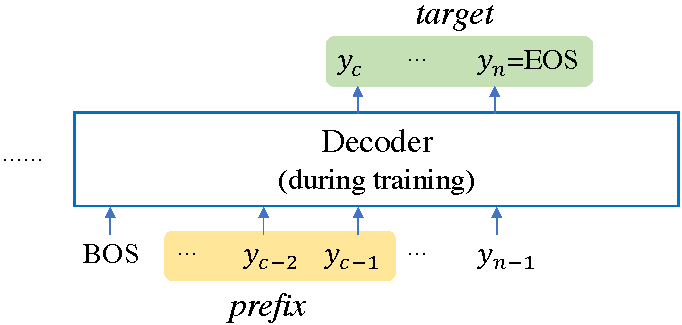
\includegraphics[scale=0.45]{decoder.pdf}
 	\caption{The decoder of a NLG model. BOS and EOS are special tokens representing the beginning and the end of the output. It's suitable for both encoder-decoder and decoder-only models.} 
 	\label{fig:decoder}
 \end{figure}
 
 
\subsection{ICL Algorithm}
\label{sec:iclalgorithm}
Since the output length varies from sample to sample, it's hard to set $c$ as a constant for all samples.
If so, samples with short outputs will be neglected when $c$ is large at the beginning, and the model will eventually bias to training samples with long outputs as they are shown more times.
In light of this, we proposed to determine $c$ sample by sample relative to their output lengths.

We define a start point $p_{start}$ and a stride $s$ for controlling $c$, where $0\leq p_{start}, s \leq 1$.
The training process starts with: 
\begin{equation}
	c = n\times p_{start}
	\label{eq:cnp}
\end{equation}
After each epoch or a number of updating steps, we validate the model on the validation set. If the performance on the validation set no longer increases, we introduce a more difficult generation task 
by removing $s$ from $p_{prev}$:
\begin{equation*}
	p_{new} = 
	\begin{cases}
	p_{prev}-s, & \text{if $p_{prev}>s$} \\
	0, & \text{else}
	\end{cases} \\
\end{equation*}
and update $c$ by Equation~\ref{eq:cnp}. The training process terminates until there are no improvements on the validation set with $c$ equaling 0.
More details are included in Algorithm~\ref{alg:picl}. %An exemplified This can be further combined with early stopping and traditional CL strategies.

\begin{algorithm}[th]
	\caption{The ICL training algorithm.}
	\label{alg:picl}
	\small
	\textbf{Input}: the model to be fine-tuned $M_{in}$, the training set $D_t$, the validation set $D_v$\\
	\textbf{Parameter}: a start point $p_{start}$, a stride $s$\\
	\textbf{Output}: the final model $M_{out}$
	\begin{algorithmic}[1] %[1] enables line numbers
		\Procedure{ICL}{$M_{in}, D_t, D_v, p_{start}, s$}	
		\State $p = p_{start}$ 
		\State $M_{out}=M_{in}$ 
			
		\For{training epoch $e=1,...$}
			%\State Update flag $f_p=False$
			\State \Comment{Training process}
			\For{training steps in an epoch}
				\State Randomly sample a batch $B$ from $D_t$
				\For{Each sample $(X, Y)$ in $B$}
					\State $c = n\times p$
					\State Calculate $L_{icl}$ by Eq.~\ref{eq:icl}
				\EndFor
				\State Update $M_{in}$ based on $\frac{1}{|B|}\sum_{|B|}L_{icl}$
			\EndFor
			\State \Comment{Validation process}
			\State Calculate $M_{in}$'s performance on $D_v$.
			\If{$M_{in}$ gets improvements on $D_v$}
				\State $M_{out} = M_{in}$
			\Else
				\State Update $p$ according to Eq.~\ref{eq:cnp}
				%\State $f_p=True$
			\EndIf
		\EndFor	
		\State \textbf{return} $M_{out}$
	
	%	\State $a\gets b$
	%	\State $b\gets r$
	%	\State $r\gets a\bmod b$
	%	\EndWhile\label{euclidendwhile}
	%	\For{\texttt{<some condition>}}
	%	\State \texttt{<do stuff>}
	%	\EndFor
	%	\State \textbf{return} $M_out$
		\EndProcedure
	\end{algorithmic}

\end{algorithm}

%The length of a prefix equals the multiplication of the percentage and the output's length.
